%%%%%%%%%%%%%%%%%%%%%%%%%%%%%%%%%%%%%%%%%%%%%%%%%%%%%%%%%%%%%%%%%%%%%%%%%%%%%%%%
%2345678901234567890123456789012345678901234567890123456789012345678901234567890
%        1         2         3         4         5         6         7         8

%\documentclass[letterpaper, 10 pt, conference]{ieeeconf}  % Comment this line out
                                                          % if you need a4paper
\documentclass[a4paper, 10pt, conference]{ieeeconf}      % Use this line for a4
                                                          % paper

\IEEEoverridecommandlockouts                              % This command is only
                                                          % needed if you want to
                                                          % use the \thanks command
\overrideIEEEmargins
% See the \addtolength command later in the file to balance the column lengths
% on the last page of the document



% The following packages can be found on http:\\www.ctan.org
%\usepackage{graphics} % for pdf, bitmapped graphics files
%\usepackage{epsfig} % for postscript graphics files
%\usepackage{mathptmx} % assumes new font selection scheme installed
%\usepackage{times} % assumes new font selection scheme installed
%\usepackage{amsmath} % assumes amsmath package installed
%\usepackage{amssymb}  % assumes amsmath package installed
\usepackage[T1]{fontenc}
\usepackage[latin1]{inputenc}
\usepackage{graphicx}

\title{\LARGE \bf
A flexible visual framework for debugging complex robotic systems
}

%\author{ \parbox{3 in}{\centering Huibert Kwakernaak*
%         \thanks{*Use the $\backslash$thanks command to put information here}\\
%         Faculty of Electrical Engineering, Mathematics and Computer Science\\
%         University of Twente\\
%         7500 AE Enschede, The Netherlands\\
%         {\tt\small h.kwakernaak@autsubmit.com}}
%         \hspace*{ 0.5 in}
%         \parbox{3 in}{ \centering Pradeep Misra**
%         \thanks{**The footnote marks may be inserted manually}\\
%        Department of Electrical Engineering \\
%         Wright State University\\
%         Dayton, OH 45435, USA\\
%         {\tt\small pmisra@cs.wright.edu}}
%}

\author{Felix Kaser$^{1}$, Bruce MacDonald$^{2}$% <-this % stops a space
%\thanks{*This work was not supported by any organization}% <-this % stops a space
\thanks{$^{1}$F. Kaser is a student in the Software Engineering Elite Graduate Program at Universit�t Augsburg, TU M�nchen and LMU M�nchen. [Add University of Auckland connection?]
        {\tt\small kaserf at in.tum.de}}%
\thanks{$^{2}$B. MacDonald is an Associate Professor at the Department of Electrical Engineering, University of Auckland,
        New Zealand
        {\tt\small b.macdonald at auckland.ac.nz}}%
}

\begin{document}

\maketitle
\thispagestyle{empty}
\pagestyle{empty}

%%%%%%%%%%%%%%%%%%%%%%%%%%%%%%%%%%%%%%%%%%%%%%%%%%%%%%%%%%%%%%%%%%%%%%%%%%%%%%%%
\begin{abstract}

[The abstract is still empty...]

Lorem ipsum dolor sit amet, consectetur adipiscing elit. Nulla hendrerit nulla eget elit dignissim fringilla. Mauris congue arcu vitae sem viverra dictum. Curabitur velit lacus, volutpat auctor vehicula a, vulputate at lacus. Phasellus laoreet varius bibendum. Nulla facilisi. Cras auctor eleifend lacus non sodales. Class aptent taciti sociosqu ad litora torquent per conubia nostra, per inceptos himenaeos. Maecenas justo urna, congue non aliquam at, vulputate in eros. Integer dictum nisi sed nulla vestibulum cursus non et odio. Donec porttitor mauris arcu, sed iaculis massa. Aenean sit amet tellus a lorem tristique lacinia. Aliquam magna massa, porttitor vel porta a, facilisis ut libero. Cras ligula magna, consequat eu cursus vitae, pretium ut leo. Curabitur cursus, tortor et euismod egestas, velit sem ultricies nisi, tempus faucibus ante lacus sit amet tortor. Nullam adipiscing posuere ante, sed elementum mi fermentum et.

\end{abstract}


%%%%%%%%%%%%%%%%%%%%%%%%%%%%%%%%%%%%%%%%%%%%%%%%%%%%%%%%%%%%%%%%%%%%%%%%%%%%%%%%
\section{INTRODUCTION}

\begin{itemize}[Introduction:]

\item initial approach to integrate tracepoints?
\item different approach to debug
\item making printf debugging better
\item current problems with robot debugging

\end{itemize}

Debugging complex robotic systems has proven to be more difficult than debugging normal (still complex) systems [check citation!] \cite{Collett2010}. One of the biggest problems when debugging robotic systems is the non-interruptible nature of robotic applications. Sometimes it is hard or even impossible to interrupt the execution of a robot without being a threat to the robot hardware, the people and the equipment in the environment where the robot is operating. For example you can not just interrupt a quad-copter in mid-flight to step through the algorithm to find a bug. [citation? rewrite? drop the example?]

One approach to address this issue is to keep two separated controllers: a low level controller that keeps the essential parts of the robot running (e.g. keep the quad-copter flying) and a high level controller that runs the application logic code which is debugged. This only solves part of the problem because developing the low level controller is still not interruptible. [citation?]

Another approach has come up in the past and it is more thorough: the concept of tracepoints is used to debug a robot application without interrupting the execution but analysing the trace post-mortem (and more recently also viewing the results live \cite{Gumbley2009}). Using tracepoints to debug a program is a highly instrumented way of debugging and does not require to modify the source code. However the tracepoints approach is quite complex and pre-execution configuration takes a substantial effort and skill, which many developers won't like to take upon them. [badly written, rewrite, no proof]

[write a paragraph about AR debugging? ---> AR Debugging covers the perception of the gobal state as seen by the robot. ROSDashboard tackles the local state of algorithms]

Because of the problems stated above many developers still use printf-debugging. It is something they can use with the skills they already have, without learning a new toolset and setting up a tracing or debugging chain[proof?]. One major downside of printf-style-debugging is the text-only representation of data. Although the developers might be used to look at (and interpret) numbers scrolling down in a console, it is not a very natural representation of the data. In this paper we [we or I?] present a new approach to improve printf-style-debugging with a special tool: ROSDashboard. The tool was developed to give developers the chance to visualize data collected with a printf-style approach how they want to. The developer can arrange widgets on a dashboard that visualize the debugged data in a more natural way. The developer can choose which visualization he prefers and suits his mental model of the data best. [unnecessary?: While printf-debugging has its downsides, there are also benefits to printf-debugging. The developer knows exactly where the printf-statements are and this makes it easy to understand the flow of a program.]

ROS (Robot Operating System) was chosen as the platform for for this tool. It is currently one of the biggest players in the sea of robot development frameworks and has a big community backing the project. The developed tool represents the first step in more research to understand how robot development works and can be improved. The tool enables future work to evaluate the underlying debugging methodology.

\section{RELATED WORK}

\begin{itemize}[Related work:]

\item ROS
\item LabView
\item tracepoints?

\end{itemize}

\subsection{ROS - Robot Operating System}
[should this subsection be shorter?]

The Robot Operating System (ROS) is an Open Source framework for complex robotic systems. The first work on ROS was done as part of the STanford Artificial Intelligence Robot (STAIR) in 2007 \cite{Quigley2007}. The original software library was called \emph{Switchyard} and had been developed at Stanford. Later the library was refined and generalized to also suit the requirements of the Personal Robot Program at Willow Garage\footnote{www.willowgarage.com} \cite{Quigley2009}. The resulting general framework has been released as Open Source \cite{Quigley2009} and a community of researchers and industry partners has grown that supports and keeps developing the framework.

ROS was built to abstract from the hardware of the robot and create modular robot software, which can run on different robots and on different machines. This makes it easier to write software for robots and distribute the work to different teams, each team focusing on one part of the robot. The modules in ROS are called \emph{nodes} and several nodes executed together are called a \emph{stack}. ROS \emph{packages} bundle nodes and stacks and are used to make software modules available to other developers. Everyone can create their own package which can be indexed by ROS so that your software modules can be found, downloaded and used by other developers. There exist many packages, nodes and stacks with implementations of algorithms for some of the most common problems in robotics (e.g. navigation, localization, joint movement, etc.) and they can easily be (re-)used.

The communication between ROS nodes can be done asynchronously through a publish/subscribe mechanism and synchronously through services. Nodes can send messages by publishing a message on a topic and receive messages by subscribing to that topic. This mechanism is really flexible and decouples the sender from the receiver. A publisher node does not need to know if there are other nodes listening and vice versa. For synchronous communication and guaranteed delivery of messages, services can be invoked. The routing is established during runtime through the ROS core. The core of ROS was kept really slim and only contains the most essential parts of the framework (such as the inter node communication). ROS can run on several machines distributed in a network, the only restriction is that every node needs to know the address of the core (master node) in order to communicate with other nodes.

The ROS client libraries currently fully support Python and C++, client libraries for Java and other languages are currently under development. ROS runs on Linux and Ubuntu is the main target distribution where it is well tested and most developers can offer support.

\subsection{LabView}

[Todo: look for papers to cite and write subection]

LabView has similar draggable widgets to make the development of systems easier.

\subsection{Tracepoints?}

[this subsection probably needs to go. I should write about AR debugging and point out the global world view AR tries to tackle and the local algorithm view rosdashboard targets -- maybe both?]

Are tracepoints still that relevant to my work to list it here?

\subsection{Related ROS tools}

[write about some graphical ros tools, especially the ones that allow you to select a topic, since the topic selection is different in rosdashboard]

\section{ROSDASHBOARD}

Design, approach, integration, ROS philosophy...

\begin{itemize}

\item design (requirements)
\item approach
\item integration
\item ROS philosophy

\end{itemize}

\subsection{Overview}
ROSDashboard is a new tool in the ROS environment. It is built to allow developers easy visualization of data streams. It is built around a central dashboard where developers can add visualization widgets with drag and drop from a toolbox. Currently there are only the most basic widgets implemented to visualize data. In future there should be added more and more widgets. This effort could come from the robot developers themselves through a simple plugin mechanism. The developers know best what widgets they need to visualize their data.

\subsection{Requirements}
Requirements (easy to install and use, simple to extend, base tool for further development and evaluation)

\subsubsection{Openness}
One of the requirements is to be open. Open in terms of Open Source but also regarding the other requirements like extendibility and adaptability. Openness helps to spread the word and gain a higher user base faster. [citation?] [badly written. rewrite]
\subsubsection{Low configuration overhead}
The goal was to create a useful tool that is easy to use and can be used by anyone without much configuration, setup or learning overhead. This contributes to a high user acceptance and a low entrance barrier [better wording?] for new users.
\subsubsection{Extendibility and adaptability}
Especially in robotics common standards are not yet defined and the variety of tools, frameworks and robot hardware is big. This means that the developed tool needs to be highly flexible. It should be easy to adapt the current system to work with any robot hardware supported by ROS and it should be designed with an open mind towards other frameworks. It also needs to be easy to reflect possible changes in the framework and underlying tools.
\subsubsection{Follow the ROS philosophy [really?]}
ROS is designed to have a really small core with as many tools build around the common core as needed. The principle is to have small tools that do one thing only but are really specialized and sophisticated in what they handle. This philosophy is followed and encouraged by the ROS core developers. It is important to follow this principle to reach a high acceptance among the ROS community and to fit in as good as possible with other tools.
\subsubsection{Integrable}
[explain current efforts of RQT and that rosdashboard should become part of it to be in the graphical ROS toolchain, but it was a moving target thus the integration is not done yet]
\subsubsection{Customization [flexibility?]}
Different developers prefer to visualize their data differently and every project is different. It is important [why important?] to create a system that can be customized by a developer to suit their preference and the targeted project best. [extend?]


\subsection{Design}
Python was chosen for ROSDashboard as target language, because it is a good match for fast prototyping and iterative development. Python's duck typing [reference] turned out to be a big help for topic introspection (see implementation details \ref{topic introspection}). Qt is used for the graphical part of the tool which also reflects the general policy in the ROS community (before Qt wxWidgets was the graphical toolkit of choice). [as of 2012, look for a reference in the wiki?]

Although the current software does not support third party widgets (in form of plugins) yet, the structure of the internal widgets is aligned to allow easy integration of such a feature in the near future. For now if a third party wants to have specialized widgets, it needs to modify the source code and add the code for widgets directly to the source tree.

ROSDashboard was developed as Open Source from the very beginning to allow external contributions and feedback. The source code is hosted on Github \footnote{http://github.com/kaserf/rosdashboard}. A prototype was announced to the ROS community and valuable feedback was gathered and documented. One of the most valuable feedback was to make ROSDashboard more generic and allow to visualize topics that publish String messages which are parsed to get the data for the visualization. This would make it possible to use ROSDashboard with existing projects that already contain extensive logging (but in text form). [move the feedback to future work section, it is not really something for the design section]

\subsection{Implementation details}
\subsubsection{Topic introspection}
\label{topic introspection}
ROS topics were originally not designed and developed as something the user or developer chooses graphically. Topics are usually set up in the code. ROSDashboard exposes the topic setup in a graphical user interface and this turned out to become a challenge since one of the requirements is to have a low configuration overhead (see requirements section [add reference]). Normally you have to select a topic name and a message data type. The data type can be one of the standard message types (wrapping the basic types like Float, Integer, String and Boolean) or a more complex message type. To access one data element of a message the "datafield" field was introduced in the graphical interface. Using Pythons duck typing and the \emph{rostopic} module it was possible to avoid the complexity of dynamically binding message types during runtime and detect the message type automatically. If a topic is not yet published (and thus the message type is not defined yet) the call to \emph{rostopic} blocks until the message type becomes known. To avoid blocking of the user interface a listener thread was implemented to wait until a topic (message type) becomes available. Avoiding to manually ask the user for a message type makes the configuration of widgets easier and faster for the user and also keeps the implementation simpler (no dynamic binding of message type classes during runtime).

[show screenshot of topic subscription dialog?]

\begin{figure}[thpb]
  \centering
  \framebox{
    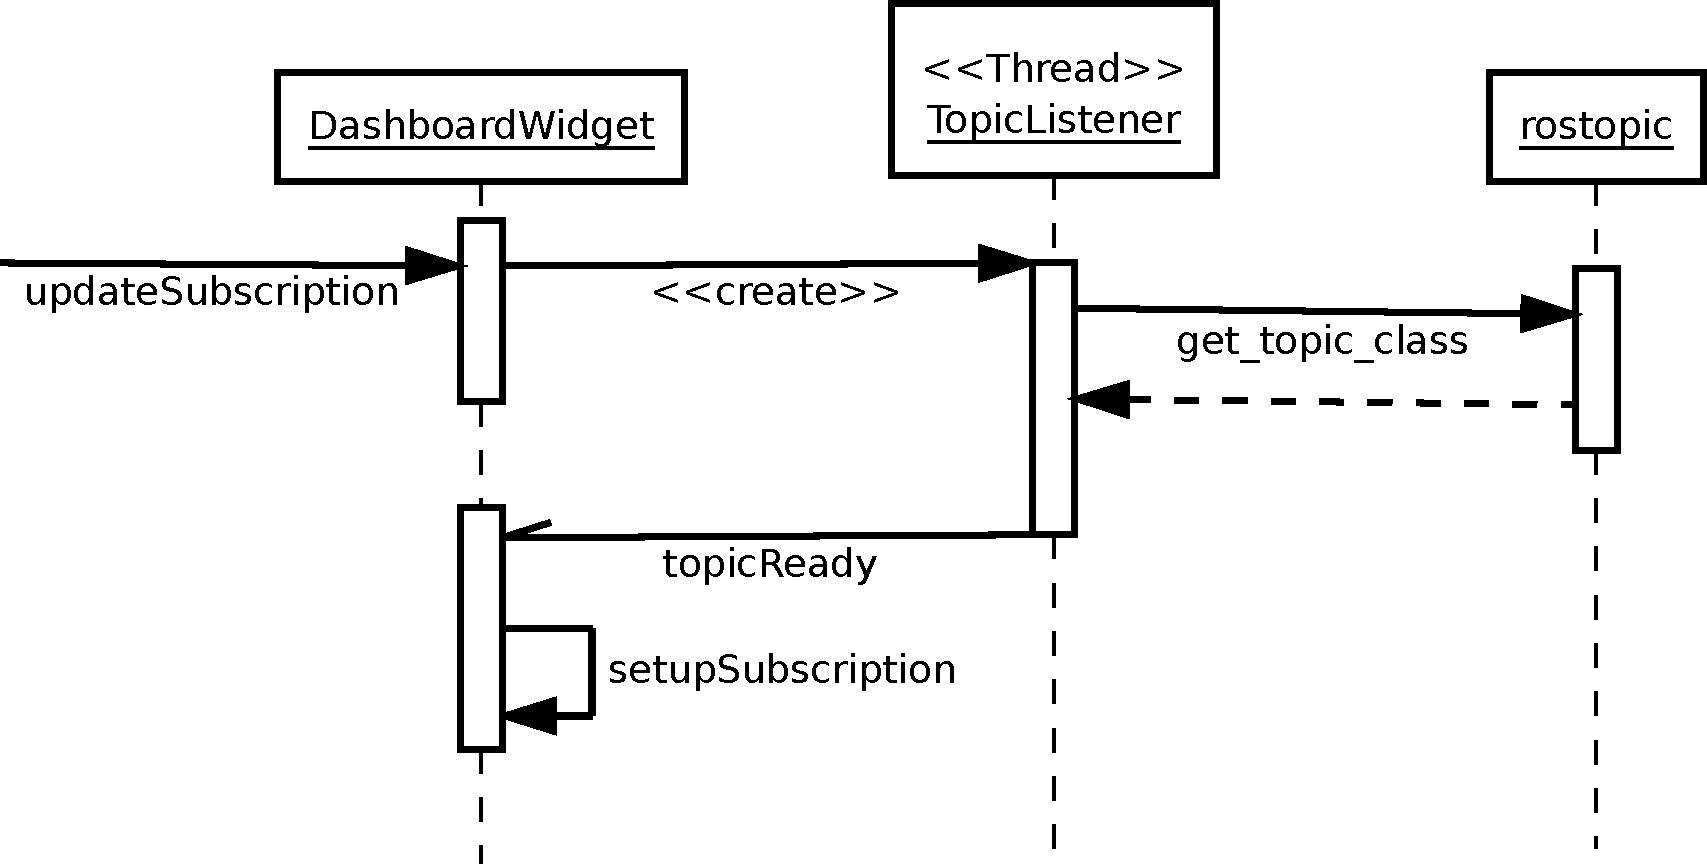
\includegraphics[scale=0.28]{diagrams/topic_subscription.pdf}
  }  
  \caption{Exemplary flow of events for updating the topic setting of a widget.}
  \label{topic subscription}
\end{figure}

The initial prototype implementation of the topic selection mechanism was developed to allow a fast and easy setup of widgets on the dashboard. In future the topic selection needs a better user interface to make it simpler to choose a topic and a datafield (and maybe the topic message type, if the topic introspection becomes to complicated). One possible solution could be a drop-down list with type-ahead auto completion and a visual representation of the message type and which fields are available to select. [highly opinionated paragraph. not sure if it makes sense to mention this]

\subsubsection{Object model}
The object model was designed to make it easy to extend ROSDashboard with more widgets. The abstract \texttt{DashboardWidget} class covers the general tasks that are the same for every widget. It provides hooks to overwrite some methods in the subclass if a widget needs to be more specific. This should allow easy integration of a plugin framework at [at? in? on?] a later stage, where third party widget developers only need to implement the specific parts of a new widget and the common tasks can be handled by the default implementation in \texttt{DashboardWidget}.

\begin{figure}[thpb]
  \centering
  \framebox{
    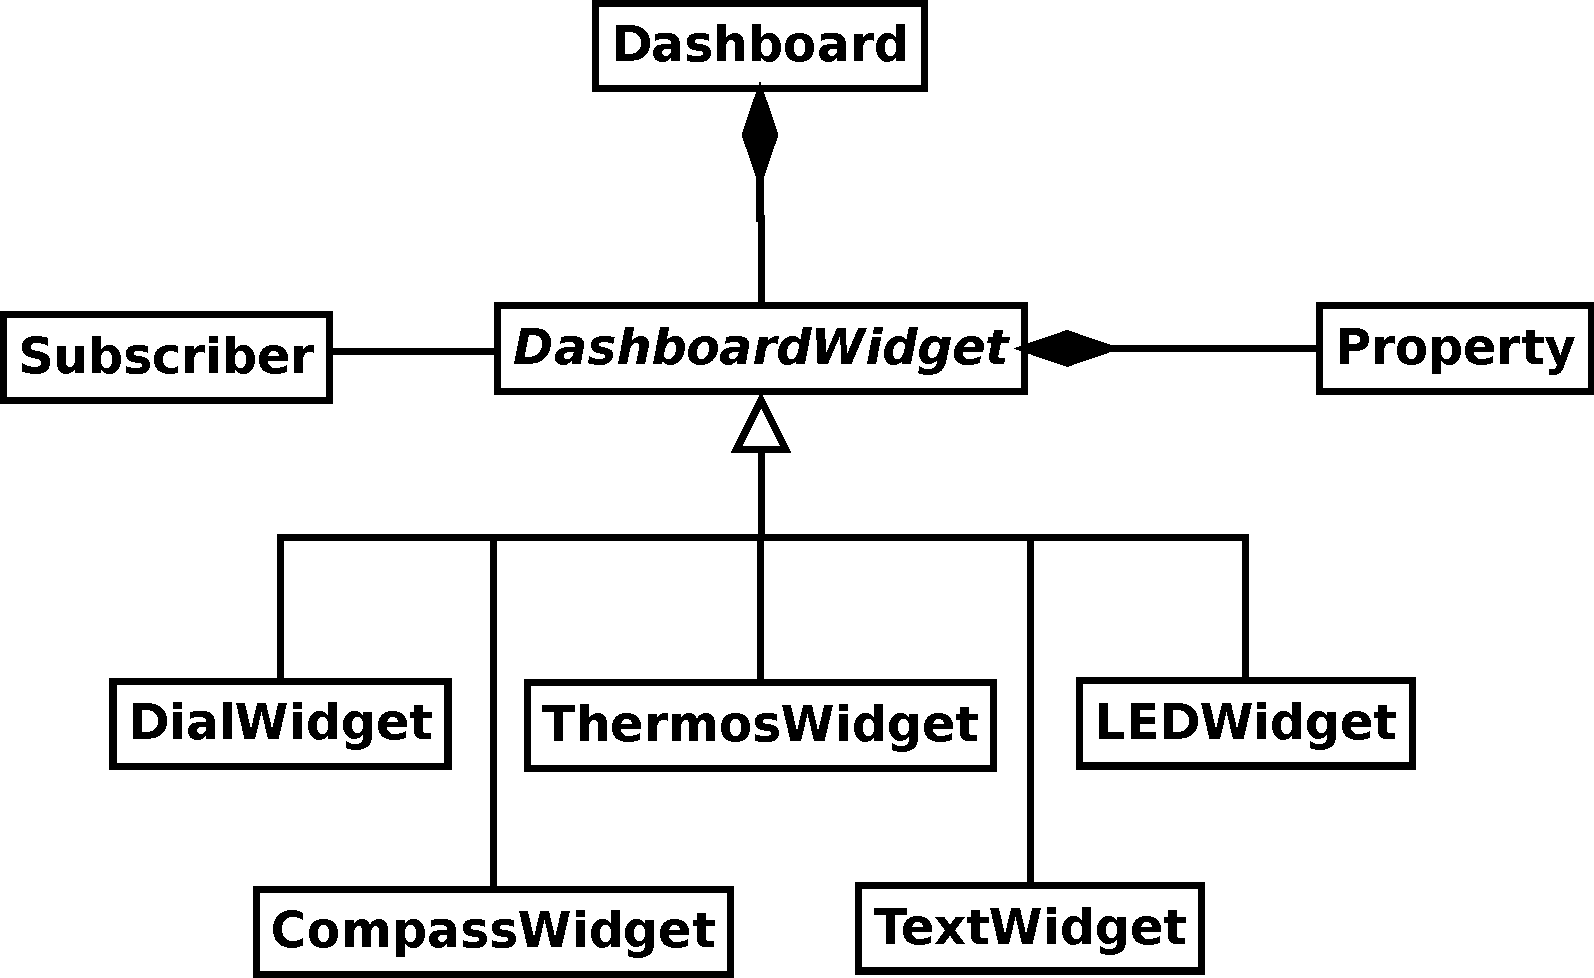
\includegraphics[scale=0.3]{diagrams/class_overview.pdf}
  }  
  \caption{Overview of the core object model structure.}
  \label{class overview}
\end{figure}

The subscription setup and the properties management are implemented in the \texttt{DashboardWidget} class as well. The main reason is to hide the technical details away from a third party plugin developer to make his life easier. The plugin developer only needs to specify which properties his widget needs and needs to implement the callback that gets called when the properties have been changed. The \texttt{DashboardWidget} supports numeric, text and float properties. If more specific properties are needed the plugin can overwrite the whole properties part and not re-use the default implementation from \texttt{DashboardWidget}.

\subsection{Open Issues}

[drop this section ---> future work]

\section{THEORETICAL CONCEPT}

This section probably is nonsense. I wanted to get into detail about the fast feedback loop, small changes to the code, how it affects the debugging and development style in general, small product increments, ...

\section{FUTURE WORK}

\begin{itemize}

\item plugin structure
\item integrate into RQT
\item more widgets
\item widget designer (small python snippets?)
\item evaluation in real project

\end{itemize}

The next steps for ROSDashboard are to integrated it into RQT and add a plugin framework to allow third parties to write widgets for ROSDashboard. A more long term plan for the project is to implement a parser that can extract data from text-based topics through regular expressions. Another long term plan is to generalize the widgets to have both subscription widgets and publisher widgets. One could have widgets that change settings of the robot and trigger special functions (a remote control for robots if you wish). [badly written, needs to be structured, extended and improved in general --> maybe split RQT integration and plugin framework into separate paragraphs]

The tool presented in this paper should be used in future to evaluate this new approach to robot debugging. It originates in printf-debugging but tries to address some of the issues of printf-debugging to increase developer productivity and make it easier to debug robot software. [add more to this paragraph and rephrase]

\section{CONCLUSIONS}

Do I need this section? What should I conclude about? Alternative approach to debugging? Fast feedback prototyping? (There was no evaluation so this section might be obsolete)

\addtolength{\textheight}{-12cm}   % This command serves to balance the column lengths
                                  % on the last page of the document manually. It shortens
                                  % the textheight of the last page by a suitable amount.
                                  % This command does not take effect until the next page
                                  % so it should come on the page before the last. Make
                                  % sure that you do not shorten the textheight too much.

%%%%%%%%%%%%%%%%%%%%%%%%%%%%%%%%%%%%%%%%%%%%%%%%%%%%%%%%%%%%%%%%%%%%%%%%%%%%%%%%



%%%%%%%%%%%%%%%%%%%%%%%%%%%%%%%%%%%%%%%%%%%%%%%%%%%%%%%%%%%%%%%%%%%%%%%%%%%%%%%%



%%%%%%%%%%%%%%%%%%%%%%%%%%%%%%%%%%%%%%%%%%%%%%%%%%%%%%%%%%%%%%%%%%%%%%%%%%%%%%%%

\section*{ACKNOWLEDGMENT}

Thank everyone :)


%%%%%%%%%%%%%%%%%%%%%%%%%%%%%%%%%%%%%%%%%%%%%%%%%%%%%%%%%%%%%%%%%%%%%%%%%%%%%%%%

%%%%% references %%%%%
\bibliographystyle{IEEEtranBST/IEEEtran}
\bibliography{bibtex/Master_Thesis}

\end{document}
